%%%%%%%%%%%%%%%%%%%%%%%%%%%%%%%%%%%%%%%%%
% Template modified from:
% Programming/Coding Assignment
% LaTeX Template
%
% Original author of template:
% Ted Pavlic (http://www.tedpavlic.com)
%%%%%%%%%%%%%%%%%%%%%%%%%%%%%%%%%%%%%%%%%

% Original author of content:
% Paul Thrane
% Please feel free to copy/edit/distribute
% The author takes no responsibility for any mistakes that might be present.

%%%%%%%%%%%%%%%%%%%%%%%%%%%%%%%%%%%%%%%%%


%----------------------------------------------------------------------------------------
%	PACKAGES AND OTHER DOCUMENT CONFIGURATIONS
%----------------------------------------------------------------------------------------

\documentclass{article}

\usepackage{fancyhdr} % Required for custom headers
\usepackage{lastpage} % Required to determine the last page for the footer
\usepackage{extramarks} % Required for headers and footers
\usepackage[usenames,dvipsnames]{color} % Required for custom colors
\usepackage{graphicx} % Required to insert images
\usepackage{listings} % Required for insertion of code
\usepackage{courier} % Required for the courier font
\usepackage{hyperref} % Make \url available

% Margins
\topmargin=-0.45in
\evensidemargin=0in
\oddsidemargin=0in
\textwidth=6.5in
\textheight=9.0in
\headsep=0.25in

\linespread{1.1} % Line spacing

% Set up the header and footer
\pagestyle{fancy}
\lhead{\sadTitle} % Top left header
%\chead{ } % Top center head
%\rhead{ } % Top right header
%\lfoot{ } % Bottom left footer
\cfoot{} % Bottom center footer
\rfoot{Page\ \thepage\ of\ \protect\pageref{LastPage}} % Bottom right footer
\renewcommand\headrulewidth{0.4pt} % Size of the header rule
\renewcommand\footrulewidth{0.4pt} % Size of the footer rule

\setlength\parindent{0pt} % Removes all indentation from paragraphs

%----------------------------------------------------------------------------------------
%	CODE INCLUSION CONFIGURATION
%----------------------------------------------------------------------------------------

\input{sadLanguageDef.txt} 	%Load part of SAD language defined in sadLanguageDef.ext

%----------------------------------------------------------------------------------------
%	NAME AND CLASS SECTION
%----------------------------------------------------------------------------------------

\newcommand{\sadTitle}{A SAD Introduction}
\newcommand{\sadDate}{May 2017}

%----------------------------------------------------------------------------------------
%	TITLE PAGE
%----------------------------------------------------------------------------------------

%\title{
%\vspace{2in}
%\textmd{\textbf{\hmwkClass:\ \hmwkTitle}}\\
%\normalsize\vspace{0.1in}\small{Due\ on\ \hmwkDueDate}\\
%\vspace{0.1in}\large{\textit{\hmwkClassInstructor\ \hmwkClassTime}}
%\vspace{3in}
%}

\title{\huge{An Introduction to Strategic Accelerator Design (SAD)}}

\author{\textbf{Paul Thrane}}
\date{
	\sadDate \\ \ \\ \ \\
	This document and accompanying source files can be found on\\
	\url{https://github.com/Vaagen/SADintro}}


%----------------------------------------------------------------------------------------

\begin{document}

\maketitle

%----------------------------------------------------------------------------------------
%	TABLE OF CONTENTS
%----------------------------------------------------------------------------------------

%\setcounter{tocdepth}{1} % Uncomment this line if you don't want subsections listed in the ToC

\newpage
\tableofcontents
\newpage

%----------------------------------------------------------------------------------------
%	Introduction
%----------------------------------------------------------------------------------------

\section{Introduction}

This document is intended primarily as a quick starting guide to SAD. As such, the structure is perhaps not the best for easy reference, although I will endeavor to make the structure as clear as possible.
There are a few other resources available, most importantly the SAD home page: \url{http://acc-physics.kek.jp/SAD/} where you will find among other things a list of many of the commands available in SAD. This list is easiest to navigate using the search function of your browser. Figure~\ref{fig:sadHomePage} points out where to find this list on the SAD home page.
\textbf{Please note:} No SAD expert has yet read through this work, there might be (and most probably is) some mistakes in the text.
% Mention Oide's presentation?

\begin{figure}[h]
	\begin{center}
	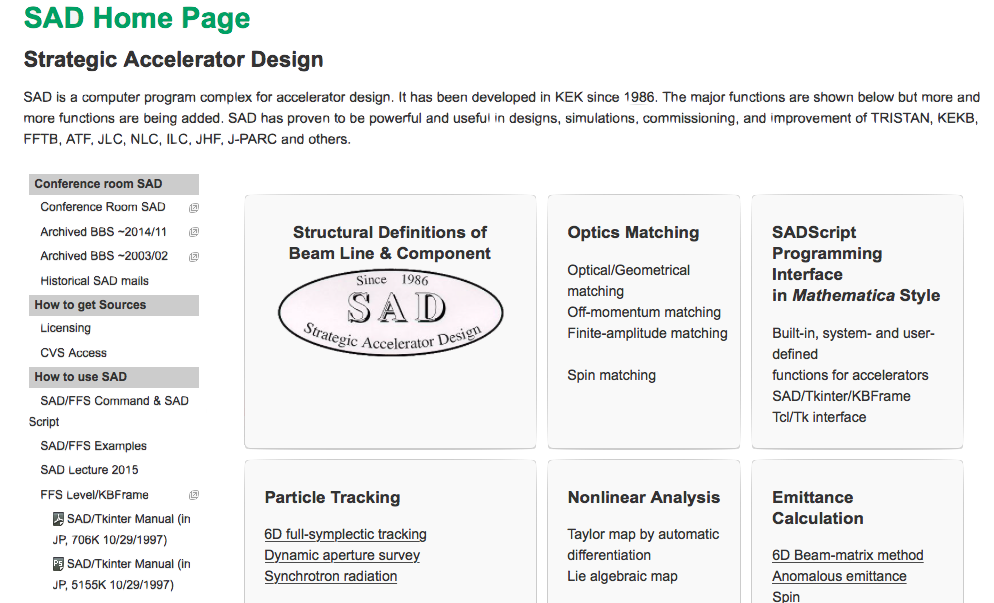
\includegraphics[width=0.75\columnwidth]{figures/sadHomePage.png}
	\end{center}
	\caption{Snapshot of the SAD home page, \url{http://acc-physics.kek.jp/SAD/}. The red arrow points out where to find a summary of many important SAD commands.}
	\label{fig:sadHomePage}
\end{figure}

\subsection{About SAD}
Strategic Accelerator Design (SAD) is a computer code developed at the Japanese High Energy Accelerator Research Organization (KEK) since 1986. It is used in the design, commissioning and operation of several accelerators including J-PARC, KEKB and now SuperKEKB. It features specialized commands for easy definition of beamlines, optics matching, particle tracking and more, in combination with a Mathematica style programming interface.
Sadly there is a lack of documentation for SAD, and therefore one often depends on seeking help from experienced users.

\subsection{Installing SAD}
An up to date repository which includes brief installation instructions on Github: \url{https://github.com/KatsOide/SAD}.
Installing TCL/TK and X11 is recommended as this allows for using the graphical functions in SAD when e.g. plotting optic functions.

\clearpage

%----------------------------------------------------------------------------------------
%	Main Level
%----------------------------------------------------------------------------------------

\section{Main Level}
SAD is divided into two levels: the main level and the FFS level. Historically, this has come about 

\subsection{Flags}


%--------------------------------------------------------
\subsection{Defining a beamline}

\subsubsection{Beam properties}
%markers and transport line

\subsubsection{Elements}
%Key elements and their key properties, include some physics
\textbf{quad}

\subsubsection{Beamline}
%markers and transport line
% Importing a lattice from another file


\clearpage
%----------------------------------------------------------------------------------------
%	FFS Level
%----------------------------------------------------------------------------------------

\section{FFS Level}

\subsection{Calculating optics}

\subsection{Matching}


Not included yet:\\
go\\
fit\\
reject\\
fix\\
free\\
var\\

elementvalues\\


\subsection{Matching Example}


%Example FODO

%Example CLIC FFS



%----------------------------------------------------------------------------------------
%	Output
%----------------------------------------------------------------------------------------

\section{Output}


%----------------------------------------------------------------------------------------
%	Tracking
%----------------------------------------------------------------------------------------

\section{Tracking}


%----------------------------------------------------------------------------------------
%	Control Structures
%----------------------------------------------------------------------------------------

\section{Control Structures}

%----------------------------------------------------------------------------------------
%	Adding errors
%----------------------------------------------------------------------------------------

\section{Adding errors}

%----------------------------------------------------------------------------------------
%	Main Level
%----------------------------------------------------------------------------------------

\section{Stuff still in need of a place}
Wildcards\\
FODO example\\
CLIC FFS example\\
Importing another file\\
Table of optical function names\\
BEAM-BEAM element\\
Luminosity calculation\\
accessing element values, LINE\\



%----------------------------------------------------------------------------------------
%	PROBLEM 2
%----------------------------------------------------------------------------------------

\section{temporary: formating code in \LaTeX}

If you want to name a function inside text, use $\backslash$texttt\{calc;\} to write  \texttt{calc;}.

\lstinputlisting{sadCode.sad}

\begin{lstlisting}
FFS;
!do some sad stuff
end;
\end{lstlisting}




%----------------------------------------------------------------------------------------

\end{document}